% !TEX root = tracking.tex
\section{Introduction}
 Currently there is a great interest both in research and industry to find methods of fast path planning for autonomous quadrotors and other vehicles. These vehicles must be able to plan and execute a dynamic trajectory in real-time without violating safety constraints. This is a very difficult challenge: the need for fast planning is generally at odds with the need for maintaining safety and robustness. In order to achieve real-time planning for any environment with static obstacles, researchers typically must use highly simplified model dynamics or kinematics, resulting in a tracking error between the planned path and the true high-dimensional system. This concept is illustrated in Figure \ref{fig:chasing}, where the path was planned using a simplified planning model, but the real vehicle cannot track this path exactly. In addition, most current planners do not consider the effect of external disturbance (e.g. wind) on the resulting tracking error. This tracking error due to the simplified dynamics and lack of disturbances can lead to unsafe situations in which the planned path may be safe, but the actual vehicle trajectory crashes into an obstacle or other unsafe region.

We propose a modular tool FASTrack: Fast and Safe Tracking, which works by modeling the navigation task as a sophisticated tracking system following a simplified planning system. Offline, a precomputed capture-avoid game between the to systems is analyzed using Hamilton Jacobi reachability analysis. This results in a function that maps the initial relative state between the two systems to the maximum possible tracking error bound between these two systems, accounting for possible worst-case external disturbances. This error bound can be thought of as a ``safety bubble" around the planning system. The precomputation also provides a safety control function that will map the current relative state to the optimal safety control for the tracking system to ``catch" the planning system. It is important to note that the offline computations are \textit{independent} of the path planned in real-time; what matters is the online relative state between the systems, not the absolute state of the path.

In the online computation, the tracking error bound is determined by the initial relative state between the planning and tracking systems. The sensed obstacles are augmented by this bound to ensure that no potentially unsafe paths can be computed. Next a path or trajectory planner uses the simplified planning model to determine the next desired position. The tracking system then finds the relative state between itself and the next desired position. This relative state is plugged into the safety control function to find the optimal control of the tracking system. This process is repeated until the navigation goal is reached. 
  

\begin{figure}
	\centering
	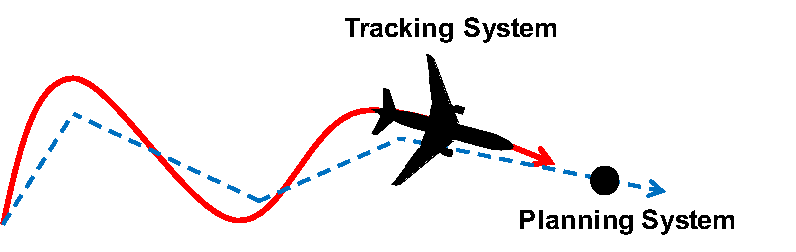
\includegraphics[width=0.47\textwidth]{fig/chasing}
	\caption{A planning system using a fast but simple model, followed by a tracking system using a dynamic model}
	\label{fig:chasing}
\end{figure}
%
FASTrack is designed to be modular and able to use in conjunction with sundry fast path and trajectory planners to add robustness and safety guarantees. In this paper we demonstrate this tool by computing a capture-avoid game between a 10-dimensional quadrotor model and a linear 3D constant-velocity model. We then plan a path using RRT through an environment with wind and static obstacles. \textcolor{red}{state results}